\documentclass[aspectratio=169]{beamer}

\usetheme{Madrid}
\usecolortheme{dolphin}
\usepackage[utf8]{inputenc}
\usepackage[T1]{fontenc}
\usepackage{amsmath,amssymb}
\usepackage{booktabs}
\usepackage{graphicx}

\setbeamertemplate{navigation symbols}{}
\setbeamertemplate{itemize items}[triangle]
\setbeamercolor{frametitle}{fg=black}
\setbeamercolor{title}{fg=black}

\title{Lag-Order Uncertainty in Set-Identified SVARs}
\subtitle{A comparative presentation of two Monte Carlo studies}
\author{Ak\i n Ayd\i n \and Ferdinand Loser}
\institute{Ludwig-Maximilian University of Munich}
\date{\today}

\begin{document}

\begin{frame}
  \titlepage
\end{frame}

\begin{frame}{Agenda}
  \tableofcontents
\end{frame}

\section{Motivation}

\begin{frame}{The central problem}
  \begin{itemize}
    \item Structural VARs are widely used for macroeconomic inference.
    \item Impulse responses depend strongly on the estimated lag structure.
    \item In finite samples, lag-order choices are uncertain and can be highly influential.
    \item Set-identified SVARs add another layer of uncertainty through the identification step.
  \end{itemize}
  \vspace{0.4cm}
  \begin{block}{Research question}
    Which estimation strategy recovers the true impulse response function most reliably when the lag order is uncertain?
  \end{block}
\end{frame}

\begin{frame}{Simulation design in a nutshell}
  \begin{itemize}
    \item A data-generating process is calibrated to the oil-market application of Kilian and Murphy (2014).
    \item VARs are estimated in repeated Monte Carlo samples.
    \item Structural IRFs are recovered using sign restrictions and the median target.
    \item Performance is evaluated by relative mean squared error.
  \end{itemize}
  \vspace{0.3cm}
  \begin{figure}
    \centering
    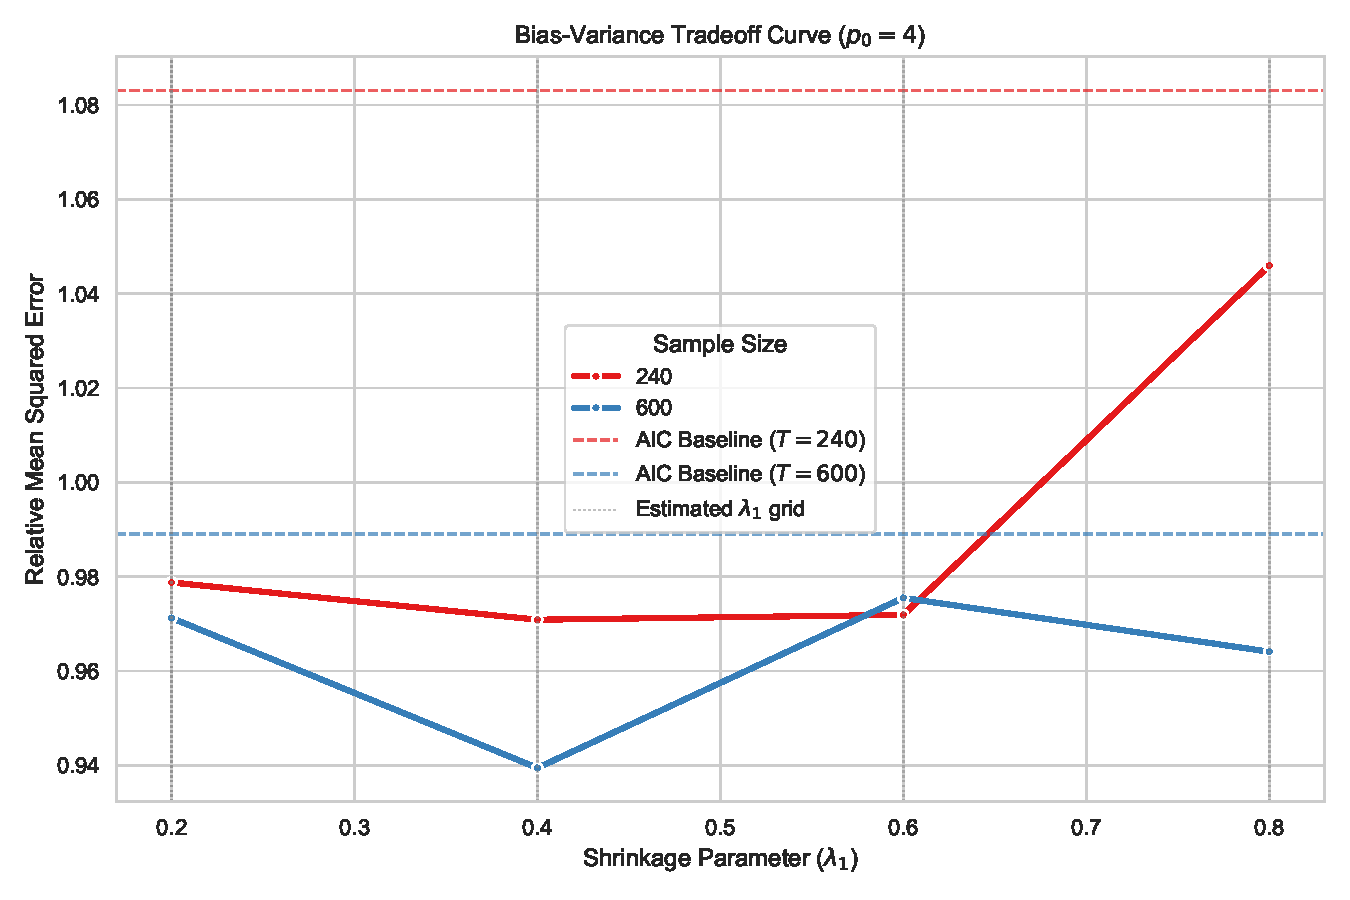
\includegraphics[width=0.8\textwidth]{Figures/Fig1_Tradeoff_Curve.pdf}
  \end{figure}
\end{frame}

\section{Paper I: BVAR}

\begin{frame}{Paper I: To Shrink or to Select?}
  \begin{itemize}
    \item Focus: comparison of information criteria and Bayesian VAR shrinkage.
    \item Main methods: AIC, BIC, HQC, and BVAR with different shrinkage hyperparameters $\lambda_1$.
    \item Main finding: AIC performs best among the classical criteria because it avoids severe underfitting.
    \item BVAR often outperforms AIC, especially when the true lag order is large.
  \end{itemize}
\end{frame}

\begin{frame}{Key results from Paper I}
  \begin{itemize}
    \item BIC and HQC are too parsimonious in finite samples and introduce substantial bias.
    \item The BVAR approach reduces variance without relying on a hard lag truncation.
    \item A moderate prior shrinkage is typically more useful than very tight shrinkage.
    \item Forecast-oriented tuning, such as MDD-based selection, does not necessarily optimize structural IRF recovery.
  \end{itemize}
\end{frame}

\begin{frame}{Takeaway from Paper I}
  \begin{block}{Conclusion}
    For structural inference, shrinkage can be more robust than selecting a single lag order when sample sizes are modest.
  \end{block}
\end{frame}

\section{Paper II: BMA}

\begin{frame}{Paper II: Hedging Against Lag Order Uncertainty}
  \begin{itemize}
    \item Focus: Bayesian model averaging as a strategy for dealing with model uncertainty.
    \item Main methods: averaging over lag orders and shrinkage specifications.
    \item Main finding: BMA reduces the sensitivity of IRF estimates to an uncertain lag order.
    \item The joint-grid BMA strategy often dominates the simple AIC benchmark.
  \end{itemize}
\end{frame}

\begin{frame}{Key results from Paper II}
  \begin{itemize}
    \item Averaging across specifications diversifies uncertainty rather than forcing a single choice.
    \item BMA performs especially well when the true lag order is high and the data are noisy.
    \item The method protects against overfitting and underfitting at the same time.
    \item Its success rests on weighting a broad set of plausible models rather than selecting one.
  \end{itemize}
\end{frame}

\begin{frame}{Takeaway from Paper II}
  \begin{block}{Conclusion}
    Model averaging is a natural response to lag-order uncertainty when the target is accurate structural inference.
  \end{block}
\end{frame}

\section{Comparison}

\begin{frame}{How the two papers relate}
  \begin{table}
    \centering
    \begin{tabular}{p{0.28\textwidth}p{0.28\textwidth}p{0.28\textwidth}}
      \toprule
      \textbf{Dimension} & \textbf{Paper I} & \textbf{Paper II} \\
      \midrule
      Main tool & BVAR shrinkage & Bayesian model averaging \\
      Core idea & Regularize the VAR & Average over competing models \\
      Advantage & Reduces variance & Hedging against model uncertainty \\
      Main limitation & Prior choice matters & Computation and weighting matter \\
      \bottomrule
    \end{tabular}
  \end{table}
\end{frame}

\begin{frame}{Shared conclusion}
  \begin{itemize}
    \item In finite samples, hard lag selection can be too brittle.
    \item Shrinkage and averaging provide robust alternatives.
    \item The best strategy depends on the objective, but both papers support a more flexible treatment of lag uncertainty.
  \end{itemize}
\end{frame}

\section{Closing}

\begin{frame}{Concluding message}
  \begin{block}{Bottom line}
    For set-identified SVARs, the most reliable inference often comes from methods that acknowledge uncertainty rather than forcing a single lag order.
  \end{block}
  \vspace{0.3cm}
  \begin{itemize}
    \item AIC remains a strong benchmark.
    \item BVAR and BMA are attractive alternatives when structural IRFs are the target.
    \item Moderate shrinkage and model averaging are especially promising in practice.
  \end{itemize}
\end{frame}

\begin{frame}{References}
  \footnotesize
  Ivanov and Kilian (2005), Kilian and Murphy (2014), Uhlig (2005), Fry and Pagan (2011), and the two papers written in this project.
\end{frame}

\end{document}
